%==============================================================================
% presentation.tex
%==============================================================================


%==============================================================================
% Configuration
%==============================================================================

% Internationalisation
\usepackage[utf8]{inputenc}
\usepackage[T1]{fontenc}
% \usepackage[ngerman]{babel}

% Different packages
\usepackage{url}
\usepackage{color,listings,paralist}
\usepackage{enumerate}
\usepackage{tabularx}
\usepackage{alltt}

% Use default Acrobat reader fonts
\usepackage{mathpazo}

% Use CM fonts (increases document size)
\usepackage{ae}

% Use images
\usepackage{graphicx}

% Configure beamer
\usetheme[secheader]{Ikhono}
\usefonttheme[onlylarge]{structurebold}
\setbeamertemplate{navigation symbols}{}

% Variables
\providecommand{\Title}{Parallel Programming}
\providecommand{\Subtitle}{Recitation Session 1}
\providecommand{\Author}{Thomas Weibel <weibelt@ethz.ch>}
\providecommand{\Institute}{Laboratory for Software Technology, \\
  Swiss Federal Institute of Technology Z\"urich}
\providecommand{\Date}{March 3, 2010}

% PDF settings
\hypersetup{
  pdftitle={\Title, \Subtitle},
  pdfauthor={\Author},
  pdfsubject={\Institute},
  pdfkeywords={parallel programming} 
}

% Titlepage
\title{\Title}
\subtitle{\Subtitle}
\author{\Author}
\institute{\Institute}
\date{\Date}

% Listings
\lstdefinestyle{Default}{
  language=Java,
  tabsize=2,
  mathescape=true,
  inputencoding=utf8,
  showstringspaces=false,
  fontadjust=true,
  basicstyle=\ttfamily,
  keywordstyle=\color{blue}\bfseries,
}
\lstdefinestyle{Number}{
  style=Default,
  numbers=left, 
  stepnumber=1, 
  numberstyle=\tiny, 
  numbersep=10pt
}
\lstset{style=Default}


%==============================================================================
% Document
%==============================================================================

\begin{document}


% Titlepage
\begin{frame}[plain]
  \titlepage
\end{frame}


\section*{Introduction}

\begin{frame}{Administration}
  \begin{itemize}
  \item Contact me if you feel lost: \url{weibelt@ethz.ch}
  \item Get the slides:
    \url{http://n.ethz.ch/~weibelt/download/parprog/}
  \item Homework is optional, everybody gets a ``testat''
  \item Past experience: students who do the homework have a good
    chance to pass the exam
  \end{itemize}

  \vspace{\stretch{1}}

  \begin{center}
    
\includegraphics[scale=0.6]{figures/java} \\
    \tiny{Source: \url{http://www.asiamex.com}}
  \end{center}
\end{frame}

\begin{frame}{Executive Summary}
  \begin{itemize}
  \item Solution to the last assignment
  \item Exceptions in Java
    \begin{itemize}
    \item Quick overview
    \item Quiz
    \end{itemize}
  \item Hints for the next assignment
  \end{itemize}

  \vspace{\stretch{1}}

  \begin{center}
    
\includegraphics[scale=0.45]{figures/dilbert-1}
  \end{center}
\end{frame}


\section{Last Assignment}

\begin{frame}{Outline}
  \tableofcontents[current]
\end{frame}

\begin{frame}[fragile]{Solution}
  \begin{lstlisting}
class Solution {
  public static void main(String[] args) {
    int i;
    int tmp;
    
    /* iterate through the argument vector */
    for (i = 0; i < args.length; i++) {
      /* convert to int and increase */
      tmp = Integer.parseInt(args[i]) + 1;
      
      /* print out the result */
      System.out.println(tmp); 
    }
  }	
}
  \end{lstlisting}
\end{frame}

\begin{frame}[fragile]{Alternative Solution}
  \begin{lstlisting}
class AlternativeSolution {
  public static void main(String[] args) {
    /* iterate through the argument vector */
    for (String arg : args) {		
      System.out.println(
      Integer.parseInt(arg) + 1
      );
    }
  } 		
}
  \end{lstlisting}
\end{frame}


\section{Exceptions}

\begin{frame}{Outline}
  \tableofcontents[current]
\end{frame}

\begin{frame}{Exceptions}
  \begin{itemize}
  \item Exceptional event
  \item If a method encounters an exception, it creates an ``exception
    object'' and hands it off to the runtime system for handling
  \item Java knows 3 types of exceptions
    \begin{itemize}
    \item Checked exceptions: Exceptions a program wants to recover
      from, eg. open a non-existing file (user input error)
    \item Errors: Exceptions beyond the program's control, eg. hard
      disk error (block cannot be read)
    \item Runtime exceptions: Violation of logic of a program,
      eg. null pointer access
    \end{itemize}
  \end{itemize}
\end{frame}

\begin{frame}{Exception Types}
  \begin{center}
    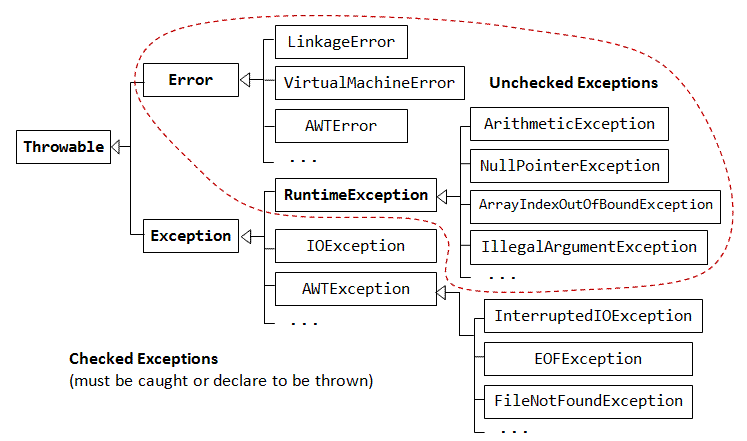
\includegraphics[width=\textwidth]{figures/exception-classes}
  \end{center}  
\end{frame}

\begin{frame}[fragile]{Throwing an Exception}
  \begin{itemize}
  \item Handing off the exception object is called throwing an
    exception
  \item Java contains the \lstinline!throw! clause
  \end{itemize}

  \vspace{\stretch{1}}

  \begin{lstlisting}
  Exception e = new Exception();
  throw (e);
  \end{lstlisting}
\end{frame}

\begin{frame}[fragile]{Try-Catch-Finally}
  Code that can throw exceptions must be enclosed in a \lstinline!try! 
  statement:
  \begin{lstlisting}
  try {
    // statements
  } 
  catch (ExceptionType1 name) {
    // handler for exceptions of type1
  } 
  catch (ExceptionType2 name) {
    // handler for exceptions of type2
  } 
  finally {
    // statements to always execute
  }
  \end{lstlisting}
  Alternative: Announce a throw in the enclosing method (see later)
\end{frame}

\begin{frame}[fragile]{Catching an Exception}
  \begin{itemize}
  \item To handle an exception it must be ``caught''
  \item Java has a \lstinline!catch! clause that will catch exceptions
    of a certain type (class):
    \begin{lstlisting}
  catch (<ExceptionType> <name>)
    \end{lstlisting}
  \item If you catch type \lstinline!X! you also catch all subtypes of
    \lstinline!X!.
  \end{itemize}
\end{frame}

\begin{frame}[fragile]{Finally}
  \begin{itemize}
  \item After the \lstinline!catch! block has finished you may want to
    ``clean'' up the state:
   \begin{lstlisting}
  try {
    ...
  } 
  finally {
    if (db != null && db.isConnected())
      db.close();
    else
      System.out.println("Not connected");
  }     
   \end{lstlisting}
 \item The \lstinline!finally! block will always be executed before
   the try statement completes
  \end{itemize}
\end{frame}

\begin{frame}[fragile]{Announcing Throws}
  \begin{lstlisting}
  class Foo {
    ...
    void bar() throws FooBarException {
      ...
      throw(new FooBarException());
    } 
  }
  \end{lstlisting}
  \vspace{\stretch{1}}

  \begin{itemize}
  \item If a method can throw an exception, you must indicate that
    there could be throws
  \item Compiler needs to prepare for possible throw
  \end{itemize}
\end{frame}

\begin{frame}[fragile]{Example}
  \begin{lstlisting}
class Example {
  public static void main(String[] args) {
    for (String arg : args) {
      try {		
        int tmp = Integer.parseInt(arg);
        if (tmp < 0)
          throw(new MyException("< 0"));
        System.out.println(tmp);    
      }    
      catch (MyException e) {
        System.out.println(e.getMessage()); 
      }
    } 
  }		
}
  \end{lstlisting}
\end{frame}

\begin{frame}[fragile]{Example: Define New Exception Type}
  New exception types can be defined by extending
  \lstinline{Exception}:

  \vspace{\stretch{1}}

  \begin{lstlisting}
  class MyException extends Exception {
    MyException(String text) {
      super(text);
    }
  }
  \end{lstlisting}
\end{frame}


\section{Exceptions Quiz}

\begin{frame}{Outline}
  \tableofcontents[current]
\end{frame}

\begin{frame}[fragile]{Quiz: Array Index}
  \begin{lstlisting}
public static void main(String[] args) {
  int[] array = new int[4];
  for (int i = 0; i < 5; i++) {
    try {
      array[i] = i;
      System.out.println(array[i]);
    } 
    catch (ArrayIndexOutOfBoundsException e) {
      System.out.println("Invalid index " 
                         + i + "\n");
    }
  }
}
  \end{lstlisting}
\end{frame}

\begin{frame}[fragile]{Quiz: Catch Order}
  \begin{lstlisting}
public static void main(String[] args) {
  try {
    throw new 
      InputMismatchException("Foobar!");
  } catch (Exception e) {
    System.out.println(e.getMessage());
  } catch (InputMismatchException e) {
    System.out.println(e.getMessage());
  }
}
  \end{lstlisting}
\end{frame}

\begin{frame}[fragile]{Quiz: Finally}
  \begin{lstlisting}
public static void main(String[] args) 
    throws Exception {
  try {
    throw new 
      Exception("I can has exception!");
  } 
  catch (Exception e) {
    System.out.println(e.getMessage());
    throw new Exception("Oh noes!");
  } 
  finally {
    System.out.println("Finally!");
  }
}
  \end{lstlisting}
\end{frame}

\begin{frame}[fragile]{Quiz: Division by Zero}
  \begin{center}
    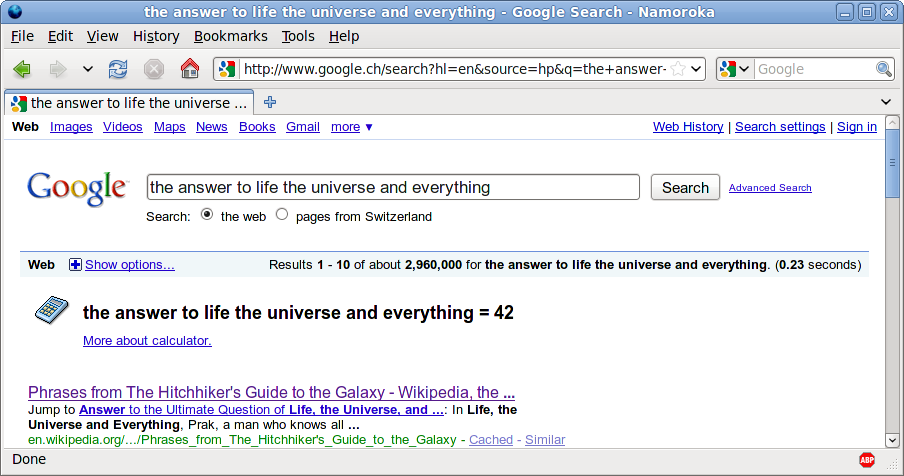
\includegraphics[width=0.8\textwidth]{figures/42}
  \end{center}

  \vspace{\stretch{1}}

  \begin{lstlisting}
public static void main(String[] args) {
  int theAnswer = 42;
  System.out.println(theAnswer / 0);
}
  \end{lstlisting}
\end{frame}


\section{New Assignment}

\begin{frame}{Outline}
  \tableofcontents[current]
\end{frame}

\begin{frame}[fragile]{Hints for the New Assignment}
  \begin{itemize}
  \item Separate \lstinline!process! method to convert and increment
  \item Define a new exception class
  \item Throw exception in case of a negative number
  \item Catch exception and print the message
  \end{itemize}

  \vspace{\stretch{1}}

  \begin{lstlisting}
  class NegValException extends Exception {
    public NegativeValueException() {
      super("Negative value -- bailing out.");
    }
  }      
  \end{lstlisting}
\end{frame}


\section*{Outro}

\begin{frame}{Summary}
  \begin{itemize}
  \item If a method encounters an exception, it creates an ``exception
    object'' and hands it off to the runtime system for handling
  \item Java knows 3 kind of exceptions: checked exceptions, errors,
    and runtime exceptions
  \item Use \lstinline{throw} to throw exceptions
  \item \lstinline{try/catch/finally} can be used to handle exceptions
  \end{itemize}

  \vspace{\stretch{1}}

  \begin{center}
    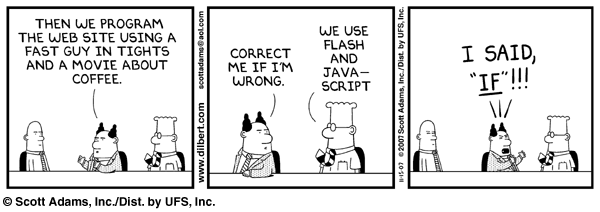
\includegraphics[scale=0.45]{figures/dilbert-2}
  \end{center}
\end{frame}

\end{document}
